% backtracking worksheet template
\documentclass[border = 1mm]{standalone}
\usepackage{tikz}
\usetikzlibrary{positioning}
\usetikzlibrary {arrows.meta}

% use default line thickness of 0.4 pt
\tikzset{backtrack/.style={rectangle,draw=black,fill=white,
inner sep=2pt,minimum height=32pt, minimum width=20mm}}
\tikzset{backtrackeq/.style={rectangle,draw=black,fill=white,
inner sep=2pt,minimum height=12pt, minimum width=20mm}}
\tikzset{backtrackstep/.style={rectangle,draw=none,fill=white,
inner sep=2pt,minimum height=12pt, minimum width=20mm}}

\begin{document}
    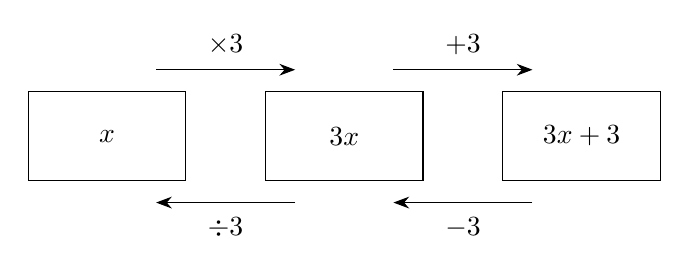
\begin{tikzpicture}
    \node[backtrack] (boxA) at (0, 0) {$x$};
    \node[backtrack] (boxB) [right=1cm of boxA] {$3x$};
    \node[backtrack] (boxC) [right=1cm of boxB] {$3x + 3$};
     
    \node (boxAr) at ([yshift=24pt,xshift=5mm]boxA) { };
    \node (boxBl) at ([yshift=24pt,xshift=-5mm]boxB) { };
    \draw [line width=0.4pt,-{Stealth[length=2mm]}] (boxAr)  --node[backtrackstep, above=3.0pt] {$\times3$} (boxBl);

    \node (boxBr) at ([yshift=24pt,xshift=5mm]boxB) { };
    \node (boxCl) at ([yshift=24pt,xshift=-5mm]boxC) { };
    \draw [line width=0.4pt,-{Stealth[length=2mm]}] (boxBr)  --node[backtrackstep, above=3.0pt] {$+3$} (boxCl);

    \node (boxCrevl) at ([yshift=-24pt,xshift=-5mm]boxC) { };
    \node (boxBrevr) at ([yshift=-24pt,xshift=5mm]boxB) { };
    \draw [line width=0.4pt,-{Stealth[length=2mm]}] (boxCrevl)  --node[backtrackstep, below=3.0pt] {$-3$} (boxBrevr);

    \node (boxBrevl) at ([yshift=-24pt,xshift=-5mm]boxB) { };
    \node (boxArevr) at ([yshift=-24pt,xshift=5mm]boxA) { };
    \draw [line width=0.4pt,-{Stealth[length=2mm]}] (boxBrevl)  --node[backtrackstep, below=3.0pt] {$\div3$} (boxArevr);
\end{tikzpicture}
\end{document}
